\part{Seminar 8 - High speed capacity of bearingless drives}

\makebox[.25\textwidth]{Martin d'Ursel}\makebox[.25\textwidth]{Margo Hauwaert}\makebox[.25\textwidth]{Aurélia Hernandez}\makebox[.25\textwidth]{Jean-Luc Timmermans}

\section{Bearingless Drives: what and why}
A bearingless drive is a drive with the bearing function fulfilled by the drive's windings. 

\begin{figure}[H]
    \centering
    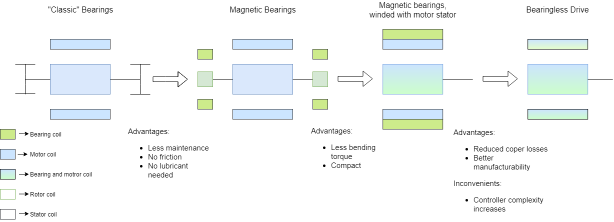
\includegraphics[scale=0.3]{bearinglessSchem.png}
\end{figure}

Progressive evolution to get to the bearingless drive: as you can see, a drive is truly bearingless when the bearing function is assured by the same coil as the motor function. 

On the third drawing, the bearing-signal is sent in the green coil while the rotor-control signal is sent in the blue coil. 

On the fourth drawing, both signals are superposed.

There are two main advangtages of bearingless drives: they can go faster (no mechanical friction) and they are compacter. 

\section{Studied topology of bearingless drive}
\subsection{Mechanical specifications of the slice disk motor}
\subsubsection{Passive and active stabilization}
Now I’m going to talk about the rotor dynamics and the stabilization of the bearingless drives of our article. The motor of our article is a bearingless permanent magnet motor. The stabilization system is made of one permanent magnet at the rotor and a combined winding system at the stator which provide the bearing force and the torque for the rotation.
The stabilization in the axial direction z and in the tilt direction alpha and Beta, tilt around x and tilt around y is passive. The rotor is stabilized passively by means of magnetic reluctance forces. The stabilization in the x and y direction is active.
Indeed, contrary to the deflection in the stable tilt direction alpha and beta and in the stable axial direction z the radial degrees of freedom x and y are unstable due to the attractive reluctance force between the stator core and the Permanent magnet at the rotor.
A displacement in the horizontal direction cause a force on the rotor also pointing in this direction thus pulling the rotor out of the center position towards the stator. 
\begin{figure}[H]
    \centering
    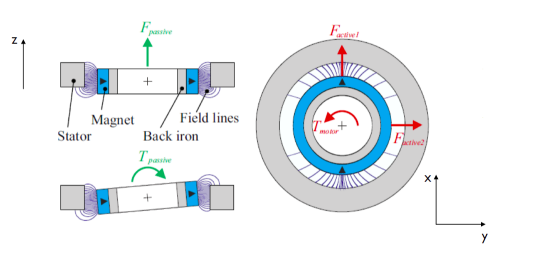
\includegraphics[scale=0.6]{passive.png}
\end{figure}


\subsubsection{Stiffness}
For a magnetic suspension as for a spring we can associate a stiffness value K and a reaction force $F=-K\cdot x$.
The controller stiffness of the bearingless unit must at least overcome the radial stiffness Krad for stabilizing the rotor. Additionally, the rotor is constituted with only one permanent magnet with two magnetic poles. Thus, the passive stiffness value is not uniform with a diametrically magnetized rotor but depend on the direction of magnetization. So, the controller stiffness must at least overcome the maximal radial stiffness. We can write $P>|Kx|$.
Defining a mean stiffness ${ k }_{ m }=\frac { { k }_{ x }+{ k }_{ y } }{ 2 } $ and a stiffness variation ratio ${ K }_{ var }=\frac { { K }_{ x } }{ { K }_{ m } } -1$.
We can re-write
$P>\left| { K }_{ m }\cdot (1+{ K }_{ var } \right| $.

\subsubsection{Resonance}
A main concern in the rotor dynamics is the different mode of resonance of the rotor and what is the resonance frequencies associate to it. To avoid serious damage on the rotor we don’t want to go in to resonance and so we want to avoid resonance frequencies. We want to avoid that the rotor speed is the same that the frequencies of resonances.
The magnetic suspension disposes of significantly smaller stiffness values than conventional sliding or roller bearings. Especially in a slotless design when large air gaps reduce the air gap flux density. The resonance frequencies are given by ${ \omega  }_{ i }=\sqrt { \frac { { K }_{ i } }{ m }  } $ for all degree of freedom i= (x, y, z, alpha, beta).
These frequencies are low at zero speed.
However, the gyroscopic effect strongly influences the critical rotors frequencies. The gyroscopic effect is the ability of a rotating body to maintain a steady direction of its axis of rotation according to the conservation of angular momentum.

The translatory mode also called cylindrical mode are not really influence by the gyroscopic effect. The translatory resonance frequencies stay constant with the speed.
The cylindrical mode is when the axe of rotation of the rotor rotate is also rotating. When the axe of rotation and the rotor rotate in the same direction we talk about forward whirl. When they are in the opposite direction we talk about backward whirl. The resonance frequencies for cylindrical modes do not varies a lot in function of the speed. These frequencies are crossed easily at low speed and are no longer a problem because we want to use the rotor at high speed. An idea to pass these rotor frequencies is to pass it with a strong acceleration.
\begin{figure}[H]
    \centering
    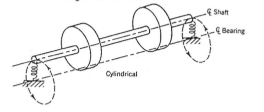
\includegraphics[scale=1]{mode1.png}
    \caption{Cylindrical mode}
    \label{cylindre}
\end{figure}

\begin{figure}[H]
    \centering
    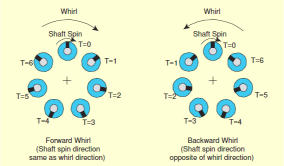
\includegraphics[scale=0.8]{backward.png}
    \caption{Backward and Forward Whirl}
\end{figure}



In contrary, the tilting mode or the conical mode change a lot with the rotational speed. The conical mode is when the axe of rotation of the rotor is stationary at the center and when the two ends of the axe trace out two circles. Again, when the whirl is in the same direction that the rotor speed we talk about forward whirl and when the whirl is in the opposite direction we talk about backward whirl. As we can see on the Campbell diagram (\ref{campbell}) due to the gyroscopic effect the resonance frequency of the conical mode increases for forward whirl direction and decrease for backward whirl direction with rising rotor speed.
with a rate depending on the ratio ri of polar to transverse moment of inertia ri=Ip/It (polar about the z axis, transvers about the x and y axis) for a flat rotor with a ratio of $ri>1$ as in the present case the resonance frequency for the forward whirl direction lies always above the current rotor frequency and is therefore never stimulated by unbalance induced synchronous disturbance. The critical backward whirl frequency is crossed easily at low rotor speeds.
\begin{figure}[H]
    \centering
    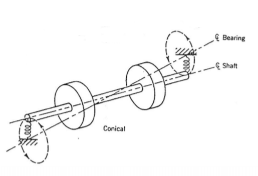
\includegraphics[scale=0.7]{mode2.png}
    \caption{Conical mode}
\end{figure}

\begin{figure}[H]
    \centering
    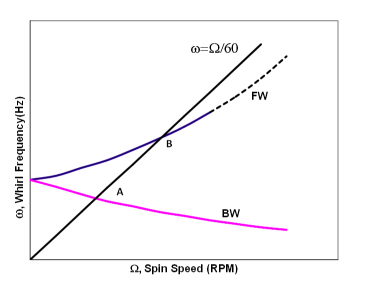
\includegraphics[scale=0.7]{cambpell.png}
    \caption{Campbell diagram}
    \label{campbell}
\end{figure}


Other problems with high speeds rotor can be the deformation due to the rotor bending mode but with the choice of a flat disk form these deformations are negligible.
\begin{figure}[H]
    \centering
    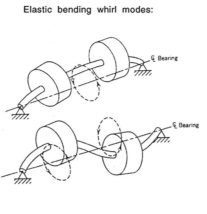
\includegraphics[scale=0.7]{bending.png}
    \caption{Bending mode}
\end{figure}


Taking into account the controller stiffness we can re-write the radial frequency
${ \omega  }_{ rad }=\sqrt { \frac { P+{ K }_{ m } }{ m }  } $
However, the anisotropic stiffness renders the whole range of 
${ \omega  }_{ rad }\cdot \sqrt { (1-\varepsilon ) } <\omega <{ \omega  }_{ rad }\cdot \sqrt { (1+\varepsilon ) } $ around the resonance frequency unstable in the undamped case.
(this interval is calculated by calculating the eigenvalue of the characteristic polynomial of the equation of motion).
In this equation w stands for the angular speeds and $\varepsilon =\sqrt { \frac { { K }_{ m }\cdot { K }_{ var } }{ P+{ K }_{ m } }  } $ descripe the ratio of stiffness anisotropy.
To suppress this unstable interval and with the choice of P we can calculate the minimum damping value Dmin to obtain stable operation over the whole rotational speed range. ${ D }_{ min }=2\cdot m\cdot { \omega  }_{ rad }\sqrt { 0.5\cdot \sqrt { 1-\epsilon  }  } $.
(this equation is calculated with the Routh-Hurwitz stability criterion on the characteristic polynomial.) 








\subsubsection{Mechanical stability}
A very important criterion for high speed operation of a motor is the ability of the rotating parts to withstand the occurring centrifugal forces which depend linearly on the mass and its radius of rotation but increase quadratically with the angular speed. 
The magnet use for the rotor of the article is rare-earth magnet. These magnets are widely applied owing to its high saturation intensity and coercive force. However, this kind of PM material has high compressive strength but low tensile strength and cannot sustain the centrifugal stress due to high speed rotation. High-remanence rare-earth magnets dispose of yield strengths of around 45-80 MPa.

\begin{figure}[H]
    \centering
    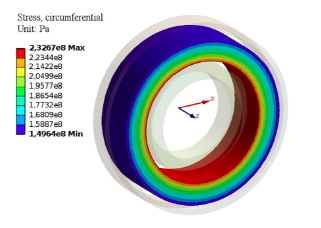
\includegraphics[scale=0.5]{stress.png}
    \caption{FEA}
    \label{FEA}
\end{figure}





On this figure \ref{FEA} a finite element analysis of a rotating permanent magnet shows the circumferential stress or tangential stress which is the most critical stress component in the rotor.
It quickly becomes clear that the brittle magnet needs to be supported by another structure. The most practicable way is to surround the permanent magnet rotor with a bandage made of high strength but magnetically non-conducting metal or fiber material. 
The carbon-fiber bandage has a high strength to weight ratio and low eddy-current losses compared to the alloy sleeve. So, carbon-fiber bandage is more often employed as the retaining sleeve in the high-speed PM motor
The use of a bandage enlarges the magnetic air gap but enhances the overall mechanical stability.
The idea behind the use of a bandage is to compensate the centrifugal stress of PMs by applying a pre-stress to the outer surface of PMs.
The prestress, the shrink range and the bandage thickness or the sleeve thickness, can be calculated analytically or by finite element analysis. The shrink range is the difference between the outer radius of the rotor and the inner radius of the sleeve.


The force diagram of the PMs is shown in this figure \ref{forcediag}. The compressive stress P2 acts on the outer surface, while P1 acts on the inner surface. P2 is decomposed into the centrifugal pressure P2w, which is produced by the centrifugal forces of the PM, and the shrinking pressure (P2-P2w) generated by magnet-sleeve interference fit. Similarly, P1 is decomposed into the centrifugal pressure P1w, and the shrinking pressure (P1-P1w).
Thus, contrary to a rotor with no retaining sleeve at zeros speed there is stress in the permanent magnet due to the compression of the sleeve.


\begin{figure}[H]
    \centering
    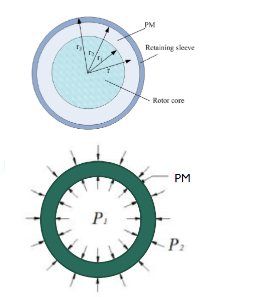
\includegraphics[scale=0.7]{sleeve4.png}
    \caption{force diagram of the PM}
    \label{forcediag}
\end{figure}




Here we can see on this graph (figure \ref{radandtang}) from a similar rotor the radial and tangential stress. Negative value indicate that the stress is compressive.
At rated speed due to the effect of centrifugal force the radial and tangential stress become less but always in compression. Indeed, The PM material has high compressive strength but low tensile strength.
By increasing the bandage thickness and the shrink range we can increase the residual contact pressure and thus increase the maximal speed. we must also take into account that the stress in the bandage is not too large and that the bandage can withstand it.
Another effect on the stress in the permanent magnet that can be take into account is the variation of temperature. With the rising of the temperature the stress in the permanent magnet retaining by carbon-fiber material increase that’s not the case for non-conducting metal material where the stress decreases slightly.
Thanks to the bandage we can obtain rotor suited for very high speed.

\begin{figure}[H]
    \centering
    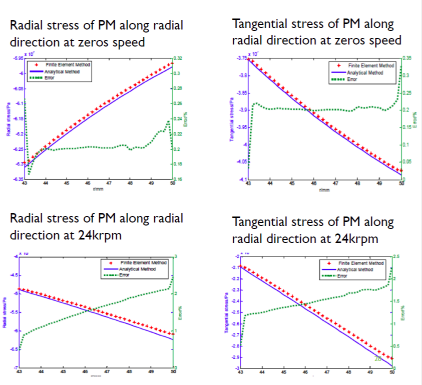
\includegraphics[scale=0.7]{sleevestab.png}
    \caption{radial and tangential stress}
    \label{radandtang}
\end{figure}


\subsection{Magnetic specifications of the slice disk motor}

\begin{itemize}
    \item sl 31: The coils at the stator are not wound over a 180 degrees while there is only 1 magnet at the rotor $\rightarrow$ reduced pitch factor 
    \item sl 32: intercepted EMF is smaller when pitch factor $!=$ 1
    \item sl 33: we have 72° between each magnetical axis (only depends on the number of poles, not how they are connected) and 108degrees coil span (this is what will influence the pitch factor) 
    \item sl 34: Why would one want to have a pitch factor <1, since that reduces the resultant EMF? Because it can reduce the harmonic content -- torque on rotor is more constant
\end{itemize}

In other papers than ours, the authors of our paper made an interesting analysis: "what if we had used 6 phases or 8 phases instead of 5 phases at the rotor?"? 
\begin{itemize}
    \item sl 36: difference between single coil (PS) and double coil (PD) 
    \item sl 37: they made a simulation model for 5pd (the one in our paper) and 6ps, validated the simulation by comparing it to the real results and than they extended the model to 5ps, 6pd, 8ps, 8pd
    \item sl 38: we observe that we obtain a higher torque using single coil then double coil. Increasing number of phases is good for PS but bad for PD
    \item sl 39: using a 5pd, we kind of have the worst case for torque production BUT we have quite a smooth torque. 
\end{itemize}


\section{Energy losses}
\subsection{Different types of losses in an electrical machine}
\begin{enumerate}
    \item Friction losses :
    \begin{itemize}
        \item Force to overcome the drag associated with the rotation of the rotor
        \item Example : friction of bearings, bushings or brushes
        \item Proportional to the rotor speed
    \end{itemize}
    \item Windage losses :
    \begin{itemize}
        \item losses sustained by a machine due to resistance of air to the rotation of the shaft
        \item Examples : armature slots, geometries that are not cylindrical or fans
        \item Proportional to the rotor speed³
        \item 	depends on design and shape of rotating object : ex : synch machine : salient pole rotors have more windage losses than non-salient poles
    \end{itemize}
    \item Iron losses / Core losses
        \begin{itemize}
        \item Losses in the magnetic paths of the motor
        \item Hysteresis losses + Eddy current losses + Anomalous losses
    \end{itemize}
    \item Copper losses : 
        \begin{itemize}
        \item Due to current flowing through the conductors of the motor : RI²
    \end{itemize}
    \item Stray losses : 
        \begin{itemize}
        \item all losses which vary with the load but which are not accurately determinable - unavoidable
    \end{itemize}
\end{enumerate}


\subsection{Stator Iron losses }
\begin{itemize}
    
\item 	In PM motors, stator iron is subject to OSCILLATING MAGNETIC FIELDS due to the spinning rotor.
\item 	Consequence :  EDDY CURRENTS and HYSTERESIS LOSSES
\item 	The effect intensified by flux concentration in the stator teeth = zones of highest flux densities are located.

\end{itemize}

\begin{enumerate}
    \item Hysteresis Losses
    \begin{enumerate}
        \item Recall of the hysteresis loop
        \begin{itemize}
            \item 	The hysteresis loop is the relationship between the induced magnetic flux density (B) and the magnetizing field (H).
            \item 	When ferromagnetic material is placed in a magnetic field, it is magnetized by induction. If we vary the magnetic intensity H of the magnetic field, the magnetic flux density B in the ferromagnetic material will not vary linearly with H.
            \item 	To form the hysteresis loop of a ferromagnetic material : 
            \begin{itemize}
                \item 	We take an unmagnetized bar of iron and magnetize it by placing it within the magnetic field of a solenoid. 
                \item 	We will magnetize the bar first in one direction and then in opposite direction by reversing the direction of current through the coil. 
                \item 	The field (H) produced by the solenoid is called the magnetizing field, or field H. It produces a magnetic flux density B in the iron bar. 
                \item 	The value of H can be increased or decreased by increasing or decreasing the current through the coil.
                \item 	So to form this loop, we simply measure the magnetic flux of a ferromagnetic material while changing the magnetizing field.

                \begin{figure}[H]
                \centering
                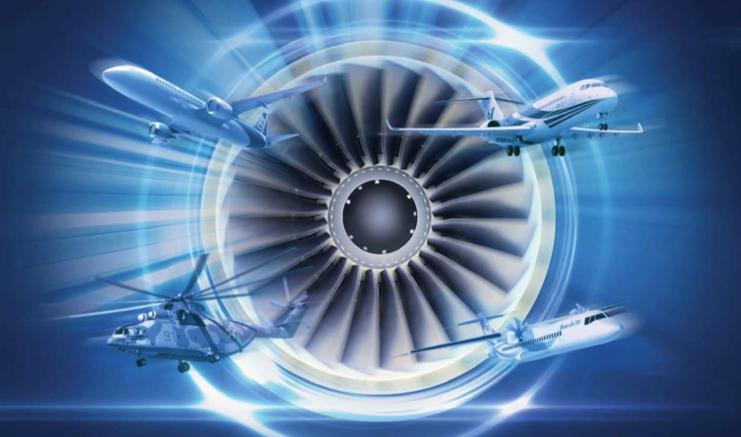
\includegraphics[scale=0.3]{1.png}
                \caption{}
                \end{figure}
            \end{itemize}
        \end{itemize}
        \item Hysteresis Loop
        \begin{figure}[H]
            \centering
            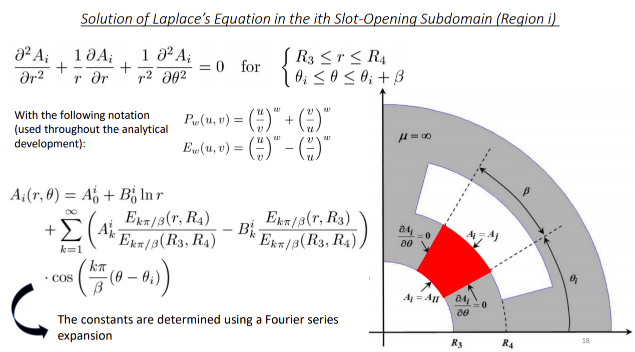
\includegraphics[scale=0.3]{2.png}
            \caption{}
        \end{figure}
        -	Current increased $\rightarrow$ magnetizing force increases $\rightarrow$ magnetic field rises $\rightarrow$ forces the domains to align
        \begin{enumerate}
            \item 	All the magnetic domains are aligned $\rightarrow$ material has reached the point of magnetic saturation. So any increase in H will not produce any increase in B.
            \item 	Current reduced to zero, so H is also decreased to zero, the magnetic flux density B decreases following a new path. B lags behind H$\rightarrow$ when H reaches zero, a  magnetic flux remains in the material $\rightarrow$ retentivity point : indicates the level of residual magnetism in the material
            \item 	Magnetic field H reversed, we increase the current in the opposite direction $\rightarrow$ flux reduced to zero $\rightarrow$ point of coercivity: ability of a ferromagnetic material to withstand an external magnetic field without being demagnetized or intensity of the applied magnetizing field required to reduce the magnetization of that material to zero after the magnetization of the sample has been driven to saturation.
            \item 	Magnetizing field H increased in negative direction $\rightarrow$ material saturated in the opposite direction 
            \item 	Reducing H to zero $\rightarrow$ residual magnetism
            \item 	Increasing H back in the positive direction: return B to zero.
            
            The magnetic flux density B always lags behind the magnetizing field H. The lagging of B behind H is called ‘hysteresis’.
        \end{enumerate}
        \item Hysteresis Losses
        \begin{itemize}
            \item A ferromagnetic material consists of local regions called ‘domains’. In an unmagnetized material, the directions of magnetization in different domains are different so that, on the average, the resultant magnetization is zero.  When we magnetize the material by placing it in an external magnetizing field, the domains that are favourably oriented wrt to the external field grow in size, and also each domain rotates so that its direction of magnetization becomes aligned with the field direction. 
            \begin{figure}[H]
                \centering
                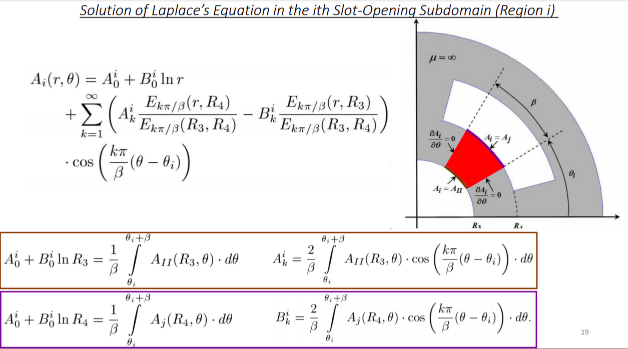
\includegraphics[scale=0.6]{3.png}
                \caption{}
            \end{figure}
            When we remove the external field H, the domain boundaries do not come back to their  position : material retains some magnetization (hysteresis effect). To make that flux zero, a coercive force is applied. That extra force = hysteresis loss.
            \item 	Steinmetz Formula : Hysteresis Loss, $P_h= k_hf B_{max}^x V$
            \begin{itemize}
                \item 	$B_{max}$ : maximum flux density [T] = [Wb/m²] = [kg/s²/A] = [V.s/m²]
                \item 	f : frequency of magnetic reversal [Hz]  = [1/s]
                \item 	V : the volume of the core [m³]
                \item 	$k_h$ : Steinmetz coefficient : material dependant constant 
                \item 	x: Steinmetz hysteresis exponent[-]
            \end{itemize}
            \item 	Energy lost per unit volume of a material in a complete cycle of magnetization is proportional to the area of the hysteresis loop.
            \item 	This knowledge has a practical application. By observing the hysteresis loop of the ferromagnetic materials, we can get an idea of its magnetic properties. This helps us in selecting the proper material for a particular application. The size and shape of the hysteresis loop of a material depend upon its nature.

        \end{itemize}
        \item Selection of magnetic materials 
        \begin{figure}[H]
            \centering
            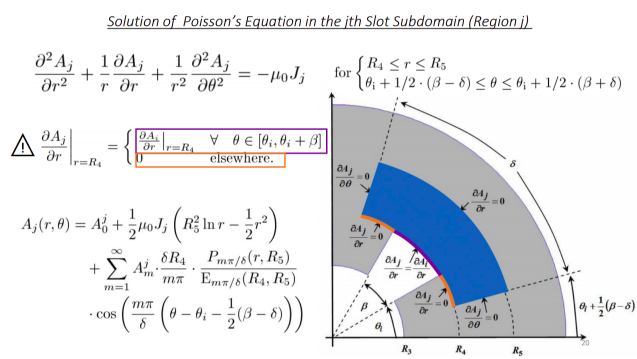
\includegraphics[scale=0.3]{4.png}
            \caption{}
        \end{figure}
        \item 	How to reduce these hysteresis losses 
        \begin{itemize}
            \item 	Hysteresis loss is undesirable in electrical machines as it produces heat, producing additional temperature rise.
            \item 	Since hysteresis loss is proportional to the area of the hysteresis loop, the loss is kept low by using materials having narrow hysteresis loops. 
            \item 	Narrow and steep hysteresis loop
            \item 	Narrow BH curve : low coercivity Hc
            \item 	Steep BH curve  : high relative permeability µr
            \item 	Solution: silicon is added to steel. For rotating electrical machines, the silicon content is at about 2\%.
        \end{itemize}
    \end{enumerate}
    \item Eddy current losses 
    \begin{enumerate}
        \item Recall of Eddy currents 
        \begin{itemize}
            \item The magnetic field surrounding a coil which is carrying AC current varies with time. This varying magnetic field induces voltages in nearby conductive materials by Faraday’s Law :  $EMF=-N d\phi/dt$. The resulting current is known as Eddy current.
            \item We often refer ourselves to conductors such us wires and coils, but it is also the case with flat conductors, as long as the object is conductive. 
            \begin{figure}[H]
                \centering
                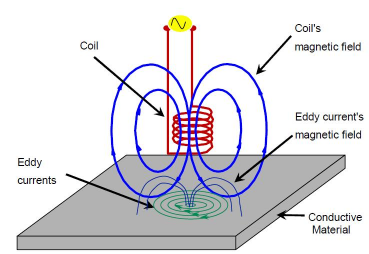
\includegraphics[scale=0.3]{5.png}
                \caption{}
            \end{figure}
            \item When a current is induced in a conductor such as a square piece of metal as shown above, the induced current often flows in small circles, in a plane that is perpendicular to the magnetic field. These currents are strongest at the surface and penetrate a short distance into the material. These current flow patterns are thought to resemble eddies in a stream, which are the tornado looking swirls of the water that we sometimes see. Because of this resemblance, these electrical currents are named Eddy currents.
            \begin{figure}[H]
                \centering
                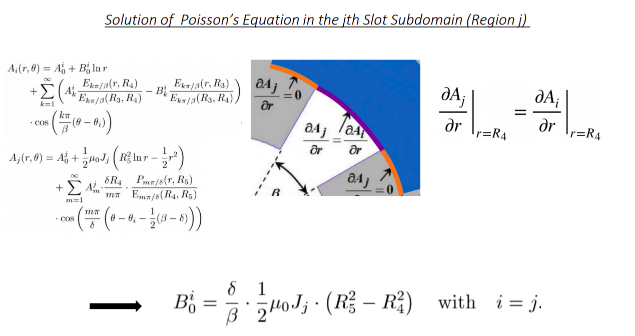
\includegraphics[scale=0.3]{6.png}
                \caption{}
            \end{figure}
        \end{itemize}
        \item In the case of a rotating electrical machines 
        \begin{itemize}
            \item In our case, a varying magnetic field appears because of the relative motion between the magnet and a nearby conductor (the iron stator).
            \item The stator iron sees then a varying magnetic field which induces eddy currents within the stator iron.
        \end{itemize}
        \item Eddy current losses
        \begin{itemize}
            \item 	Eddy currents results into heating up the core because of $RI^2$ losses. Additional power is required to make up this loss $\rightarrow$ unwanted power loss
	        \item Eddy current losses can be calculated using an empirical formula :  $P_e=k_e V (f .t .B_{max}  )^2$
	        \begin{itemize}
	            \item $k_e$ : material dependant constant
	            \item V: material volume [$m^3$]
	            \item f: supply frequency [Hz]
	            \item $B_max$ : the maximum flux density [T]
	            \item t : the lamination thickness
	        \end{itemize}
        \end{itemize}
        \item Material Solution : How to reduce the Eddy current losses
        \begin{itemize}
            \item 	To reduce the eddy current loss, the resistance of the core should be increased. In other words, low reluctance should be retained.

            \item 	We split the core in n subsections, and insulate them from each other. The e.m.f induced will be divided n because the flux linked to the core will be divided by n $\rightarrow$ Eddy currents in each length will be reduced. 

            \item 	The core is then made of laminations of iron, that is small sheets of steel and each lamination being insulated from the others. Because the laminations sheet are thin, they will have relatively high resistance. 
            
            \begin{figure}[H]
                \centering
                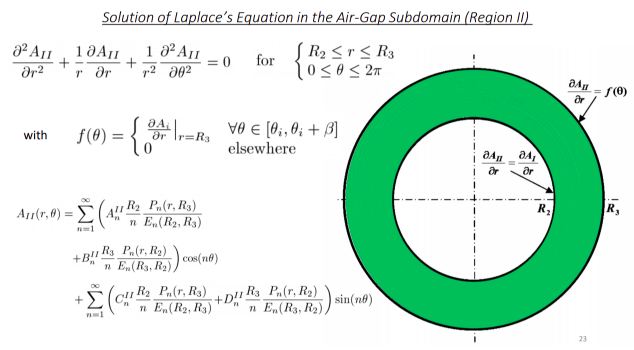
\includegraphics[scale=0.3]{7.png}
                \caption{}
            \end{figure}
            
            \item 	Each lamination sheet will have an eddy current circulating within its area and the sum of the individual eddy currents flowing through the laminations are very small compared to the case where a single solid iron core is used.
            \item 	So if we have a large number of sheets, also called laminations, the Eddy currents will be reduced.
            \item 	Rotating machines are made of thin laminations (0.35- 0.5 mm) insulated from each other to reduce Eddy current losses.
        \end{itemize}
    \end{enumerate}
    \item Solutions to decrease the power losses : 
        \begin{itemize}
            \item Stator material selection : seen above 
            \item Stator topology : 
            \begin{itemize}
                \item 	We know that a changing magnetic field induces core losses. And the effect of the changing magnetic field is intensified by the flux concentration in the stator teeth. The stator teeth being a zone where the highest flux densities are located.
                \item 	So the stator teeth are a source of further losses because they are typically permeated by a higher rotor field and also cause higher field harmonics. A slotless design do not show these additional losses $\rightarrow$ slotless design advantageous for high speed drives 
                \item 	A quick overview on the differences between slotted and slotless motors. The slotted motors have a higher torque density and high acceleration while slotless have smoother torque so slotless motors are preferable when high accuracy is needed.
            \end{itemize}
\begin{figure}[H]
   \begin{minipage}[c]{.46\linewidth}
      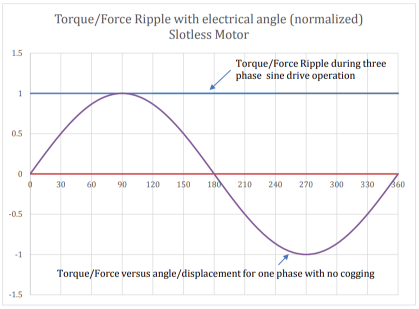
\includegraphics[scale=0.3]{slotless.png}
   \end{minipage} \hfill
   \begin{minipage}[c]{.46\linewidth}
      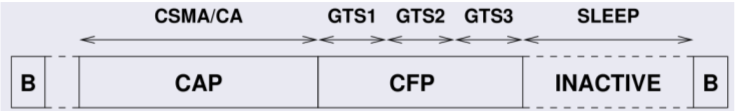
\includegraphics[scale=0.3]{slotted.png}
   \end{minipage}
\end{figure}

    \end{itemize}
\end{enumerate}





\subsection{Rotor eddy current losses}
Rotor Eddy Current Losses not significant compare to total machine loss BUT removing heat from rotor is more difficult than removing heat from stator.  Accurate prediction of rotor losses important especially at high speed. If the rotor gets too hot, the magnets could demagnetise, and this is rather bad. 

Eddy currents in the rotor are due to a variety of factors:
\begin{itemize}
    \item in a slotted machine, discontinuous permeability as the magnets move past each slot of stator. indeed, even if the magnetic flux emited from the rotor is constant, the variation in permeability between the windings and the slots from the machine will cause eddy current in the rotor because the percieved flux will vary. This problem can be solved by using a slotless design. So we use one
    \item Eddy curents are also caused by harmonics, wich are obviously varying with time. Harmonics are even bigger if we use square current control, so we will use a sinusoidal one. Also, the pitch factor has a big impact on harmonics, so we choose a pitch factor that offsets the third order harmonic. 
    \item note: laminating the rotor to counter eddy current like its is done in a lot of application is not a good idea here, because it would be too difficult to machine and would compromise the mechanical stability of the structure. 
\end{itemize}
\section{design recap}

\begin{figure}[H]
    \centering
    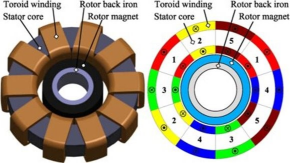
\includegraphics[scale=0.7]{design.png}
    \caption{radial and tangential stress}
\end{figure}

The final design of the windings are as depicted hereabove. the Design is slotless (avoid eddy curents in rotor), has an optimal pitch factor (to avoid harmonics), has 5 phases (for good control) and has toroid windings. the toroid design is not necessary, as the "external" windings are not used. however, it helps reduce coil heads drasticly, and provides the same magnetic equivalent for the inside circle. 

\section{Loss measurements}

(slide 63 and 64) 
We measure the effects from a rotor that is connected to a shaft and rotates at fixed speed, on a stator that is actually free to rotate (put in bearingless drives). The rotation of the stator will cause the activation of a lever, that exerts a force on a mass. That exerted force can be measured (and thus the exerted torque of the stator). 

Aerodynamic losses: we let the rotor turn very very fastly, we measure the effect of the "wind" created by the rotor on a dummy stator. That dummy stator has exactly the same form as the real stator but is not made of unmagnetic materials

Then we do the same test but using the "real" stator. Now we have the effect of aerodynamics and of magnetics. The torque experienced by the stator is the same torque that the rotor has to overcome when the stator is fixed.



\section{Control}
The choice of high value for controller-induced stiffness P and damping reduce the influence of magnetic rotor anisotropy and minimize rotor deflections. Unfortunately, this renders the system prone to sensor noise which will be amplified just like the desired signals and worse, calls for Increased bearing currents. 
While this might not be a problem when crossing the relatively low radial resonance frequency 
At around 50 Hz, the maximum current can be quickly reached when unbalance-caused deflection needs to be corrected at higher speeds. 
Due to inevitable unbalance the axis of geometry of the rotor always differs to the axis of inertia. At low speed the rotor is controlled to spin around his axis of geometry. But as the speed increase the rotor “want” more and more to move and to spin around his axis of inertia and the demanded bearing forces, necessary for keeping the rotor spinning around this axis of geometry, increase. The more the forces increase and the more the necessary current increases. And so, the current limit can easily be reached at high speed.
Fortunately, the active magnetic bearing allows to make some adjustment. As the rotor passes the critical speed, its axis of rotation shifts from its axis of geometry to the axis of inertia which is differ due to unbalance. Allowing the rotor to spin around this new axis of rotation avoids to spend a lot of bearing power on forcing it back to the old one. This, however, can only be done if the orbiting movement of the rotor can be tolerated.


This can be done by using a Notch filter; The idea is to suppress via the notch filter the rotor synchronous position signal which describe this unbalance orbit. The ideal desired filter has an infinitely sharp notch at the exact rotor frequency in order to not influence the remaining signal spectrum (Figure \ref{notch1}). In the real filter there is of course a certain gab band. 
The goal of the notch filter is to suppress the position sensor signal after the critical speed and not before. Implementing a hard tun-on turn-off as the rotational speed passes a certain threshold level result in a sudden change of the position error signal. This sudden variation of bearing forces can lead to high rotor deflection. The solution is to constantly use the filter and vary the notch frequency as a consequence of the current rotor speed.
This means that the notch frequency in case of rotational speeds far below the filter threshold speed stays constant, leaving the position signal completely unchanged in magnitude and phase. As the rotor speed approaches the threshold value, the position signal due to the rotor orbit is increasingly damped and finally completely suppressed as the rotor speed passes the filter threshold level.
So, after the critical frequency the notch frequency continue to follow the rotor speed.

\begin{figure}[H]
    \centering
    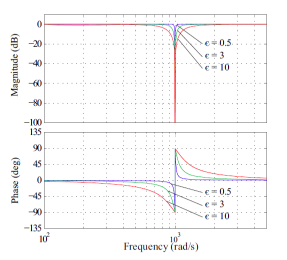
\includegraphics[scale=0.7]{notch1.png}
    \caption{Bode diagram of the notch filter}
    \label{notch1}
\end{figure}


Explanation of the FIGURE \ref{notch4}
\begin{enumerate}[label=\Alph*)]
\item The resulting rotor movement does not show stable behaviour. In the 3D- orbit plot in it can clearly be seen, that the rotor never starts to levitate but is instead bounced from one side of the emergency bearing to the other. 
\item According to the 3D- orbit plot stable and smooth operation has been achieved. In however, the increasing phase current shows the drawback of a fixed axis of rotation as unbalance effects gain importance with rising speed.
\item The phase current in is dramatically reduced since the bearing forces for keeping the rotor spinning around its axis of geometry are no longer needed. The sudden change in the position error, however, provokes a disturbance of the rotor's orbit at around 15.000rpm.
\item Soft switching algorithm is implemented. Regarding the phase current the transient region from unfiltered to filtered position signal is clearly visible shortly before the threshold value is reached. a consequence, the small disturbance in the rotor orbit which can be observed in case of hard switching does not occurs in this case.
\end{enumerate}

\begin{figure}[H]
    \centering
    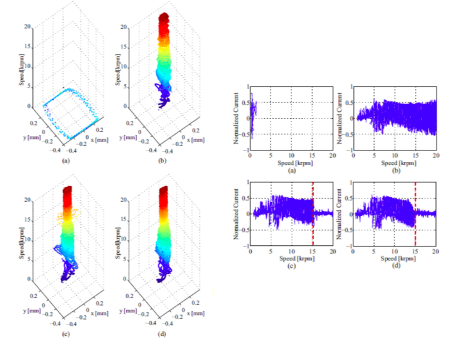
\includegraphics[scale=0.6]{notch4.png}
    \caption{}
    \label{notch4}
\end{figure}
